% Practice Test 03 — Virginia Edition
% Questions: 30 (21 MC + 9 SA)
% Generated by scripts/generate_practice_tests.py

\begin{practiceQuestion}{1-4-q29}{gsa}
\begin{questionText}
Use the graph to write an equation for the proportional relationship. Then predict $y$ when $x = 10$.

\begin{center}
\begin{tikzpicture}[scale=0.7]
  \draw[step=1,gray!20,thin] (0,0) grid (7,7);
  \draw[thick,->] (0,0) -- (7.5,0) node[right]{\small $x$};
  \draw[thick,->] (0,0) -- (0,7.5) node[above]{\small $y$};
  \foreach \x in {1,...,7} \draw (\x,0.07) -- (\x,-0.07) node[below]{\tiny \x};
  \foreach \y in {1,...,7} \draw (0.07,\y) -- (-0.07,\y) node[left]{\tiny \y};
  \draw[thick,funBlue] (0,0) -- (7,4.9);
  \fill[funBlue] (0,0) circle (2.5pt);
  \fill[funBlue] (5,3.5) circle (2.5pt) node[above left]{\small $(5, 3.5)$};
\end{tikzpicture}
\end{center}
\end{questionText}
\correctAnswer{$y = 0.7x$; when $x = 10$, $y = 7$}
\explanation{$k = \frac{3.5}{5} = 0.7$. Equation: $y = 0.7x$. At $x = 10$: $y = 0.7 \times 10 = 7$.}
\end{practiceQuestion}

\begin{practiceQuestion}{2-1-q12}{mc}
\begin{questionText}
$63$ is $90\%$ of what number?
\end{questionText}
\choiceA{$56.7$}
\choiceB{$67$}
\choiceC{$70$}
\choiceD{$72$}
\correctAnswer{C}
\explanation{Divide: $63 \div 0.90 = 70$.}
\end{practiceQuestion}

\begin{practiceQuestion}{2-2-q11}{mc}
\begin{questionText}
A recipe uses $3$ cups of sugar out of $12$ cups of ingredients total. What percent is sugar?
\end{questionText}
\choiceA{$20\%$}
\choiceB{$25\%$}
\choiceC{$30\%$}
\choiceD{$36\%$}
\correctAnswer{B}
\explanation{$\frac{3}{12} = \frac{p}{100}$. Cross-multiply: $12p = 300$. Divide: $p = 25\%$.}
\end{practiceQuestion}

\begin{practiceQuestion}{2-3-q25}{sa}
\begin{questionText}
A store's revenue went from $\$8{,}000$ to $\$6{,}400$. Find the percent decrease.
\end{questionText}
\correctAnswer{$20\%$}
\explanation{Change: $8{,}000 - 6{,}400 = 1{,}600$. Percent decrease: $1{,}600 \div 8{,}000 = 0.20 = 20\%$.}
\end{practiceQuestion}

\begin{practiceQuestion}{2-7-q26}{gmc}
\begin{questionText}
The table below shows four students' estimates and the actual values. Which student had the smallest percent error?

\begin{center}
\begin{tabular}{|l|c|c|}
\hline
\textbf{Student} & \textbf{Estimated} & \textbf{Actual} \\
\hline
Amy & $48$ & $50$ \\
\hline
Ben & $22$ & $20$ \\
\hline
Cara & $78$ & $80$ \\
\hline
Dan & $33$ & $30$ \\
\hline
\end{tabular}
\end{center}
\end{questionText}
\choiceA{Amy ($4\%$)}
\choiceB{Ben ($10\%$)}
\choiceC{Cara ($2.5\%$)}
\choiceD{Dan ($10\%$)}
\correctAnswer{C}
\explanation{Amy: $2/50 = 4\%$. Ben: $2/20 = 10\%$. Cara: $2/80 = 2.5\%$. Dan: $3/30 = 10\%$. Cara has the smallest error.}
\end{practiceQuestion}

\begin{practiceQuestion}{3-2-q18}{mc}
\begin{questionText}
What value of $n$ makes $(-9) + n = -2$ true?
\end{questionText}
\choiceA{$-11$}
\choiceB{$-7$}
\choiceC{$7$}
\choiceD{$11$}
\correctAnswer{C}
\explanation{$(-9) + n = -2$ means $n = -2 - (-9) = -2 + 9 = 7$.}
\end{practiceQuestion}

\begin{practiceQuestion}{3-3-q26}{gmc}
\begin{questionText}
The number line shows a subtraction rewritten as addition. What is the original subtraction problem?

\begin{center}
\begin{tikzpicture}
  \draw[thick,->] (-8.5,0) -- (4.5,0);
  \foreach \x in {-8,...,4} \draw (\x,0.1) -- (\x,-0.1) node[below] {\footnotesize $\x$};
  \fill[black] (-2,0) circle (3pt);
  \draw[thick,->,funGreen] (-2,0.5) -- (4,0.5);
  \node[above,funGreen] at (1,0.5) {$+6$};
  \node[below=12pt] at (-2,-0.1) {\footnotesize start};
\end{tikzpicture}
\end{center}
\end{questionText}
\choiceA{$(-2) - 6 = -8$}
\choiceB{$(-2) - (-6) = 4$}
\choiceC{$4 - 6 = -2$}
\choiceD{$4 - (-2) = 6$}
\correctAnswer{B}
\explanation{The arrow shows $(-2) + 6 = 4$. Adding $6$ is the same as subtracting $-6$, so the original subtraction is $(-2) - (-6) = 4$.}
\end{practiceQuestion}

\begin{practiceQuestion}{3-4-q19}{sa}
\begin{questionText}
What is $-\dfrac{2}{3} + \dfrac{1}{4}$?
\end{questionText}
\correctAnswer{$-\dfrac{5}{12}$}
\explanation{Common denominator $12$: $-\frac{8}{12} + \frac{3}{12} = -\frac{5}{12}$.}
\end{practiceQuestion}

\begin{practiceQuestion}{4-3-q12}{mc}
\begin{questionText}
Expand $\frac{2}{3}(9x + 6)$.


\fractionBar{2}{3}
\end{questionText}
\choiceA{$6x + 6$}
\choiceB{$6x + 4$}
\choiceC{$3x + 4$}
\choiceD{$18x + 4$}
\correctAnswer{B}
\explanation{$\frac{2}{3} \times 9x = 6x$ and $\frac{2}{3} \times 6 = 4$. Result: $6x + 4$.}
\end{practiceQuestion}

\begin{practiceQuestion}{4-4-q11}{mc}
\begin{questionText}
Factor $-12y + 8$.
\end{questionText}
\choiceA{$4(-3y + 2)$}
\choiceB{$-4(3y + 2)$}
\choiceC{$-4(3y - 2)$}
\choiceD{Both A and C}
\correctAnswer{D}
\explanation{$4(-3y + 2) = -12y + 8$ \checkmark. Also $-4(3y - 2) = -12y + 8$ \checkmark. Both are valid factored forms.}
\end{practiceQuestion}

\begin{practiceQuestion}{5-4-q16}{mc}
\begin{questionText}
A student estimates that the solution to $0.48x + 3.1 = 12.7$ is about $x = 20$. Is this estimate reasonable?
\end{questionText}
\choiceA{Yes, the exact answer is $20$}
\choiceB{Yes, the exact answer is close to $20$}
\choiceC{No, the exact answer is about $10$}
\choiceD{No, the exact answer is about $33$}
\correctAnswer{A}
\explanation{Subtract $3.1$: $0.48x = 9.6$. Divide by $0.48$: $x = 20$. The estimate is exactly correct.}
\end{practiceQuestion}

\begin{practiceQuestion}{5-5-q13}{mc}
\begin{questionText}
Which value of $x$ is a solution to $4x - 1 > 11$?
\end{questionText}
\choiceA{$x = 2$}
\choiceB{$x = 3$}
\choiceC{$x = 4$}
\choiceD{$x = 1$}
\correctAnswer{C}
\explanation{Solve: $4x > 12$, so $x > 3$. Only $x = 4$ satisfies $x > 3$. Check: $4(4) - 1 = 15 > 11$ \checkmark.}
\end{practiceQuestion}

\begin{practiceQuestion}{5-6-q02}{mc}
\begin{questionText}
Which graph represents $x \leq -2$?
\end{questionText}
\choiceA{Open circle at $-2$, shade left}
\choiceB{Closed circle at $-2$, shade right}
\choiceC{Closed circle at $-2$, shade left}
\choiceD{Open circle at $-2$, shade right}
\correctAnswer{C}
\explanation{$x \leq -2$: closed circle (includes $-2$) and shade left (values less than or equal to $-2$).}
\end{practiceQuestion}

\begin{practiceQuestion}{6-1-q05}{mc}
\begin{questionText}
A scale drawing uses $1$ cm $= 4$ m. A room is $5$ cm by $3$ cm on the drawing. What is the actual area of the room?
\end{questionText}
\choiceA{$15$ m$^2$}
\choiceB{$60$ m$^2$}
\choiceC{$192$ m$^2$}
\choiceD{$240$ m$^2$}
\correctAnswer{D}
\explanation{Actual dimensions: $5 \times 4 = 20$ m and $3 \times 4 = 12$ m. Area: $20 \times 12 = 240$ m$^2$.}
\end{practiceQuestion}

\begin{practiceQuestion}{6-2-q27}{gmc}
\begin{questionText}
The two rectangles below represent the same room drawn at two different scales. The original uses $1$ cm $= 6$ m. What scale does the new drawing use?

\begin{center}
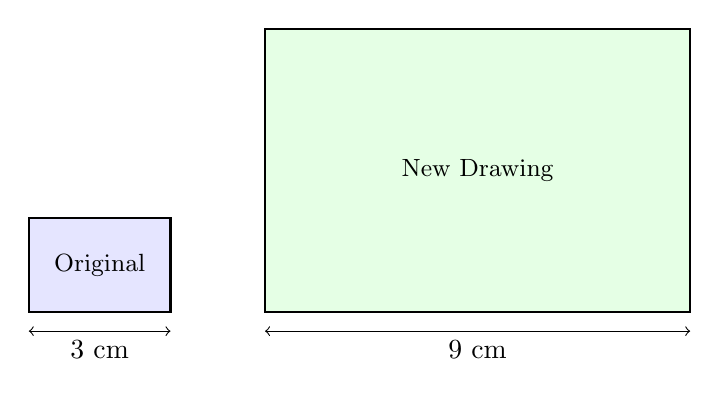
\begin{tikzpicture}[scale=0.6]
  % Original
  \draw[thick,fill=blue!10] (0,0) rectangle (3,2);
  \node at (1.5,1) {\small Original};
  \draw[<->] (0,-0.4) -- (3,-0.4);
  \node[below] at (1.5,-0.4) {$3$ cm};
  % New
  \draw[thick,fill=green!10] (5,0) rectangle (14,6);
  \node at (9.5,3) {\small New Drawing};
  \draw[<->] (5,-0.4) -- (14,-0.4);
  \node[below] at (9.5,-0.4) {$9$ cm};
\end{tikzpicture}
\end{center}
\end{questionText}
\choiceA{$1$ cm $= 2$ m}
\choiceB{$1$ cm $= 3$ m}
\choiceC{$1$ cm $= 6$ m}
\choiceD{$1$ cm $= 18$ m}
\correctAnswer{A}
\explanation{Scale ratio: $9 \div 3 = 3$. The new drawing is $3$ times bigger. Actual length: $3 \times 6 = 18$ m. New scale: $18 \div 9 = 2$ m per cm.}
\end{practiceQuestion}

\begin{practiceQuestion}{6-5-q20}{sa}
\begin{questionText}
A rectangular prism has a base of $6$ cm by $4$ cm and a height of $10$ cm. It is sliced parallel to the base. What are the dimensions of the cross-section?
\end{questionText}
\correctAnswer{$6$ cm by $4$ cm}
\explanation{A cut parallel to the base of a rectangular prism produces a rectangle identical to the base: $6$ cm by $4$ cm.}
\end{practiceQuestion}

\begin{practiceQuestion}{6-6-q25}{sa}
\begin{questionText}
Two lines intersect. One of the four angles is $(4x + 20)°$. Its adjacent angle is $(6x - 10)°$. Find the value of $x$.
\end{questionText}
\correctAnswer{$17$}
\explanation{Adjacent angles at an intersection are supplementary: $4x + 20 + 6x - 10 = 180$. Combine: $10x + 10 = 180$. Solve: $10x = 170$, $x = 17$.}
\end{practiceQuestion}

\begin{practiceQuestion}{6-7-q01}{mc}
\begin{questionText}
Point $A(3, 5)$ is translated right $4$ and down $2$. What are the coordinates of $A'$?
\end{questionText}
\choiceA{$(7, 7)$}
\choiceB{$(7, 3)$}
\choiceC{$(-1, 7)$}
\choiceD{$(-1, 3)$}
\correctAnswer{B}
\explanation{Right $4$: $3 + 4 = 7$. Down $2$: $5 - 2 = 3$. So $A'(7, 3)$.}
\end{practiceQuestion}

\begin{practiceQuestion}{6-8-q05}{mc}
\begin{questionText}
A flagpole casts a $24$-ft shadow. At the same time, a $6$-ft person casts an $8$-ft shadow. How tall is the flagpole?
\end{questionText}
\choiceA{$12$ ft}
\choiceB{$18$ ft}
\choiceC{$32$ ft}
\choiceD{$20$ ft}
\correctAnswer{B}
\explanation{Set up: $\frac{6}{8} = \frac{h}{24}$. Cross-multiply: $8h = 144$. Divide: $h = 18$ ft.}
\end{practiceQuestion}

\begin{practiceQuestion}{7-4-q06}{mc}
\begin{questionText}
An L-shaped room can be split into a $10$ ft by $8$ ft rectangle and a $4$ ft by $6$ ft rectangle. What is the total floor area?
\end{questionText}
\choiceA{$56$ ft$^2$}
\choiceB{$80$ ft$^2$}
\choiceC{$104$ ft$^2$}
\choiceD{$128$ ft$^2$}
\correctAnswer{C}
\explanation{$10 \times 8 = 80$ ft$^2$. $4 \times 6 = 24$ ft$^2$. Total: $80 + 24 = 104$ ft$^2$.}
\end{practiceQuestion}

\begin{practiceQuestion}{7-5-q30}{gsa}
\begin{questionText}
A box without a lid is shown below. What is the total surface area (including the bottom but NOT the top)?

\begin{center}
\begin{tikzpicture}[scale=0.4]
  % Front face
  \draw[thick,funBlue,fill=funBlue!10] (0,0) -- (8,0) -- (8,5) -- (0,5) -- cycle;
  % Top (open — dashed)
  \draw[thick,dashed,gray] (0,5) -- (3,7) -- (11,7) -- (8,5);
  % Right face
  \draw[thick,funBlue,fill=funBlue!15] (8,0) -- (11,2) -- (11,7) -- (8,5) -- cycle;
  % Labels
  \draw[thick,funRed,<->] (0,-0.7) -- (8,-0.7);
  \node[below,funRed] at (4,-0.7) {$8$ cm};
  \draw[thick,funRed,<->] (11.5,2) -- (11.5,7);
  \node[right,funRed] at (11.5,4.5) {$5$ cm};
  \draw[thick,funRed,<->] (8,-0.7) -- (11,-0.7+2);
  \node[below right,funRed] at (9.5,0) {$3$ cm};
\end{tikzpicture}
\end{center}
\end{questionText}
\correctAnswer{$134$ cm$^2$}
\explanation{Bottom: $8 \times 3 = 24$ cm$^2$. Front and Back: $2(8 \times 5) = 80$ cm$^2$. Two sides: $2(3 \times 5) = 30$ cm$^2$. Total (no top): $24 + 80 + 30 = 134$ cm$^2$.}
\end{practiceQuestion}

\begin{practiceQuestion}{7-6-q14}{mc}
\begin{questionText}
A rectangular prism is $8$ in by $5$ in by $4$ in. Another is $10$ in by $4$ in by $4$ in. Which has more volume and by how much?
\end{questionText}
\choiceA{First prism, by $10$ in$^3$}
\choiceB{Second prism, by $10$ in$^3$}
\choiceC{First prism, by $20$ in$^3$}
\choiceD{They have the same volume}
\correctAnswer{D}
\explanation{First: $8 \times 5 \times 4 = 160$ in$^3$. Second: $10 \times 4 \times 4 = 160$ in$^3$. They have the same volume.}
\end{practiceQuestion}

\begin{practiceQuestion}{7-7-q02}{mc}
\begin{questionText}
Which formula gives the volume of a cylinder?
\end{questionText}
\choiceA{$V = 2\pi rh$}
\choiceB{$V = \pi r^2 h$}
\choiceC{$V = \pi r^2$}
\choiceD{$V = \frac{1}{3}\pi r^2 h$}
\correctAnswer{B}
\explanation{The volume of a cylinder is $V = \pi r^2 h$ (area of the circular base times the height).}
\end{practiceQuestion}

\begin{practiceQuestion}{8-1-q24}{sa}
\begin{questionText}
A random sample of $100$ out of $4{,}000$ residents found that $45$ support a new library. Predict how many residents support it.
\end{questionText}
\correctAnswer{$1{,}800$}
\explanation{$\frac{45}{100} = 45\%$. Then $45\%$ of $4{,}000 = 1{,}800$.}
\end{practiceQuestion}

\begin{practiceQuestion}{8-3-q19}{sa}
\begin{questionText}
Group A: mean $65$, MAD $5$. Group B: mean $75$, MAD $5$. How many MADs apart are the means?
\end{questionText}
\correctAnswer{$2$ MADs}
\explanation{Difference: $75 - 65 = 10$. Divide by MAD: $\frac{10}{5} = 2$ MADs.}
\end{practiceQuestion}

\begin{practiceQuestion}{8-4-q04}{mc}
\begin{questionText}
Which measure of variability focuses on the middle $50\%$ of the data?
\end{questionText}
\choiceA{Range}
\choiceB{Mean}
\choiceC{Interquartile range (IQR)}
\choiceD{Median}
\correctAnswer{C}
\explanation{IQR $= Q_3 - Q_1$ measures the spread of the middle $50\%$ of the data.}
\end{practiceQuestion}

\begin{practiceQuestion}{8-5-q13}{mc}
\begin{questionText}
Data: $45, 48, 52, 55, 55, 58, 61, 63$. Which is the correct stem-and-leaf plot?
\end{questionText}
\choiceA{Stems: $4, 5, 6$; Row $4$: $5\;\;8$; Row $5$: $2\;\;5\;\;5\;\;8$; Row $6$: $1\;\;3$}
\choiceB{Stems: $4, 5, 6$; Row $4$: $5\;\;8$; Row $5$: $5\;\;5\;\;2\;\;8$; Row $6$: $3\;\;1$}
\choiceC{Stems: $45, 48, 52$; no leaves}
\choiceD{Stems: $4, 5$; Row $4$: $5\;\;8$; Row $5$: $2\;\;5\;\;5\;\;8\;\;1\;\;3$}
\correctAnswer{A}
\explanation{Stems are tens digits ($4, 5, 6$), leaves are ones digits listed in order. Only choice A has correct stems and ordered leaves.}
\end{practiceQuestion}

\begin{practiceQuestion}{9-3-q27}{gmc}
\begin{questionText}
The frequency table shows the results of spinning a spinner $100$ times. Which color has an experimental probability closest to $\frac{1}{4}$?

\begin{center}
\begin{tabular}{|c|c|}
\hline
\textbf{Color} & \textbf{Frequency} \\
\hline
Red & $30$ \\
\hline
Blue & $24$ \\
\hline
Green & $18$ \\
\hline
Yellow & $28$ \\
\hline
\end{tabular}
\end{center}
\end{questionText}
\choiceA{Red}
\choiceB{Blue}
\choiceC{Green}
\choiceD{Yellow}
\correctAnswer{B}
\explanation{$\frac{1}{4} = 0.25$. Blue: $\frac{24}{100} = 0.24$, which is closest to $0.25$.}
\end{practiceQuestion}

\begin{practiceQuestion}{9-6-q01}{mc}
\begin{questionText}
What is the probability of flipping two coins and getting heads on both?
\end{questionText}
\choiceA{$\frac{1}{2}$}
\choiceB{$\frac{1}{3}$}
\choiceC{$\frac{1}{4}$}
\choiceD{$\frac{3}{4}$}
\correctAnswer{C}
\explanation{Sample space: HH, HT, TH, TT ($4$ outcomes). Only HH is heads-heads. $P = \frac{1}{4}$.}
\end{practiceQuestion}

\begin{practiceQuestion}{9-7-q20}{sa}
\begin{questionText}
You roll a die $90$ times to simulate a $\frac{1}{6}$ probability event. How many times do you expect the event to occur?
\end{questionText}
\correctAnswer{$15$}
\explanation{$90 \times \frac{1}{6} = 15$.}
\end{practiceQuestion}
